\documentclass{llncs}
\usepackage{url}
\usepackage{proof}
\usepackage{amssymb}
\usepackage{stmaryrd}
\usepackage{listings}
\usepackage{graphicx}

\newcommand{\inkscape}[2][1.5]{
\begin{center}
\scalebox{#1}{
\includegraphics{diagrams/#2}
}
\end{center}
}

%subcode-inline{bnf-inline} name langRev
%! swap+ = \mathit{swap}^+
%! swap* = \mathit{swap}^*
%! dagger =  ^{\dagger}
%! assocl+ = \mathit{assocl}^+
%! assocr+ = \mathit{assocr}^+
%! assocl* = \mathit{assocl}^*
%! assocr* = \mathit{assocr}^*
%! identr* = \mathit{uniti}
%! identl* = \mathit{unite}
%! dist = \mathit{distrib}
%! factor = \mathit{factor}
%! (o) = \fatsemi
%! (;) = \fatsemi
%! (*) = \times
%! (+) = +
%! foldB = fold_B
%! unfoldB = unfold_B
%! foldN = fold_N
%! unfoldN = unfold_N
%! trace+ = \mathit{trace}^{+}
%! trace* = \mathit{trace}^{\times}
%! :-* = \multimap^{\times}
%! :-+ = \multimap^{+}
%! emptyset = \emptyset

%subcode-inline{bnf-inline} regex \{\{(((\}[^\}])|[^\}])*)\}\} name main include langRev
%! [^ = \ulcorner
%! ^] = \urcorner
%! [v = \llcorner
%! v] = \lrcorner
%! Union = \bigcup
%! in = \in
%! |-->* = \mapsto^{*}
%! |-->> = \mapsto_{\ggg}
%! |-->let = \mapsto_{let}
%! |--> = \mapsto
%! <--| = \mapsfrom
%! |- = \vdash
%! <=> = \Longleftrightarrow
%! <-> = \leftrightarrow
%! ~> = \leadsto
%! ::= = ::=
%! /= = \neq
%! vi = v_i
%! di = d_i
%! si = s_i
%! sj = s_j
%! F = \texttt{F}
%! T = \texttt{T}
%! forall = \forall
%! exists = \exists
%! empty = \emptyset
%! eta = \eta
%! where = \textbf{where}
%! epsilon = \varepsilon
%! least = \phi
%! loop+ = loop_{+}
%! loop* = loop_{\times}
%! CatC = {\mathcal C}
%! CatA = {\mathcal A}
%! gamma = \gamma
%! {[ = \{
%! ]} = \}
%! elem = \in
%! dagger = ^\dagger
%! alpha = \alpha
%! beta = \beta
%! rho = \rho
%! @@ = \mu
%! @ = \,@\,
%! langRev = \Pi
%! langRevT = \Pi^{o}
%! langRevEE = \Pi^{\eta\epsilon}_{+}
%! bullet = \bullet
%! * = \times
%! langRevT = \Pi^{o}
%! langRevTF = \Pi^{o/}

%%%%%%%%%%%%%%%%%%%%%%%%%%%%%%%%%%%%%%%%%%%%%%%%%%%%%%%%%%%%%%%%%%%%%%%%%%%%%

\begin{document}
\title{Fractional Types}
\author{}
\institute{}
\maketitle

%%%%%%%%%%%%%%%%%%%%%%%%%%%%%%%%%%%%%%%%%%%%%%%%%%%%%%%%%%%%%%%%%%%%%%%%%%%%%
\begin{abstract}
?
\end{abstract}

%%%%%%%%%%%%%%%%%%%%%%%%%%%%%%%%%%%%%%%%%%%%%%%%%%%%%%%%%%%%%%%%%%%%%%%%%%%%%
\section{Introduction} 

%%%%%%%%%%%%%%%%%%%%%%%%%%%%%%%%%%%%%%%%%%%%%%%%%%%%%%%%%%%%%%%%%%%%%%%%%%%%%
\section{Syntax and Semantics}

We can turn the above system of isomorphisms into a (reversible)
programming language by simply providing a syntax for each of the
isomorphisms. For each isomorphism, we introduce two
\emph{combinators} corresponding to the left-to-right and
right-to-left directions. 

\begin{definition}[Primitive {{langRev}} Combinators]
\label{def:primitives-langRev}

%subcode{bnf} include main
%! columnStyle = rrcll
%  zeroe :&  0 + b &<->& b &: zeroi
%  swap+ :&  b1 + b2 &<->& b2 + b1 &: swap+
%  assocl+ :&  b1 + (b2 + b3) &<->& (b1 + b2) + b3 &: assocr+
%  unite :&  1 * b &<->& b &: uniti
%  swap* :&  b1 * b2 &<->& b2 * b1 &: swap*
%  assocl* :&  b1 * (b2 * b3) &<->& (b1 * b2) * b3 &: assocr*
%  dist0 :&  0 *b &<->& 0  &: factor0
%  dist :& (b1 + b2) * b3 &<->& (b1 * b3) + (b2 * b3) &: factor
  
\end{definition}

Each line of this table is to be read as the definition of one or two
combinators. For example, corresponding to the \textit{identity of
  multiplication} ({{1*b<->b}}) we have the two combinators
{{unite:1*b<->b}} (reading the isomorphism from left to right) and
{{uniti:b<->1*b}} (reading the isomorphism from right to left). These
combinators are inverses of each other.  Each of the two cases of
commutativity defines one combinator that is its own inverse.

Now that we have primitive combinators we need some means of composing
them. We construct the composition combinators out of the congruence
closure of basic isomorphisms. Thus we have program constructs that
witness reflexivity {{id}}, symmetry {{sym}}, transitivity {{(;)}},
and two parallel composition combinators, one for sums {{(+)}} and one
for pairs {{(*)}}.

\begin{definition}[Composition in {{langRev}}]
%subcode{proof} include main
%@  ~
%@@ id : b <-> b 
%
%@ c : b1 <-> b2
%@@ sym c : b2 <-> b1
%
%@ c1 : b1 <-> b2
%@ c2 : b2 <-> b3
%@@ c1(;)c2 : b1 <-> b3
%----
%@ c1 : b1 <-> b3
%@ c2 : b2 <-> b4
%@@ c1 (+) c2 : b1 + b2 <-> b3 + b4
%
%@ c1 : b1 <-> b3
%@ c2 : b2 <-> b4
%@@ c1 (*) c2 : b1 * b2 <-> b3 * b4
\end{definition}

\noindent To summarize the syntax of our language {{langRev}} is as follows.

\begin{definition}[Syntax of {{langRev}}]
\label{def:langRev}
We collect our types, values, and combinators, to get the full language
definition:
%subcode{bnf} include main
% value types, b ::= 0 | 1 | b+b | b*b 
% values, v ::= () | left v | right v | (v,v) 
%
% combinator types, t ::= b <-> b
% primitive combinators, iso ::= zeroe | zeroi | swap+ | assocl+ | assocr+ 
%                   &|& unite | uniti | swap* | assocl* | assocr* 
%                   &|& dist0 | factor0 | dist | factor 
% combinators, c ::= iso | id | sym c | c (;) c | c (+) c | c (*) c 
\end{definition}

By design, for each combinator {{c : b1 <-> b2}}, there is an
\emph{adjoint} {{c^dagger : b2 <-> b1}} acting in the reverse direction. 

\begin{definition}[Adjoints {{c^dagger}}]
 The adjoint of a combinator {{c}} is defined by {{c^dagger}} as
 follows. For primitive combinators {{c}}, {{c^dagger}} is given by
 the inverse in Def.~\ref{def:primitives-langRev}. For the remaining
 combinators, we have:
%subcode{opsem} include main
% id^dagger &=& id
% (sym c)^dagger &=& c
% (c1(;)c2)^dagger &=& c2^dagger (;) c1^dagger
% (c1 (+) c2)^dagger &=& c1^dagger (+) c2^dagger
% (c1 (*) c2)^dagger &=& c1^dagger (*) c2^dagger
which essentially amounts to reversing the order of sequential composition.
\end{definition}

The semantics of {{langRev}} is given using two mutually recursive
interpreters: one going forward and one going backwards. The use of
{{sym}} switches control from one evaluator to the other. 

\begin{definition}[Operational Semantics of {{langRev}}]
\label{def:operational-langRev}
Given a program {{c : b1 <-> b2}} in {{langRev}}, we can run it in the
forward direction by supplying it with a value {{ v1 : b1 }} and in
the backwards direction by supplying it with a value {{v2 : b2}}. The
forward evaluator {{evalF}} and the backwards evaluator {{evalB}} are
given below. Since there are no values that have the type {{0}}, the
clauses for the combinators {{zeroe}}, {{zeroi}}, {{dist0}} and
{{factor0}} omit the impossible cases.

\paragraph*{Forward Evaluator:}

%subcode{opsem} include main
%! columnStyle = rcl
% evalF zeroe (right v) &=& v
% evalF zeroi v &=& right v
% evalF swap+ (left v) &=& right v
% evalF swap+ (right v) &=& left v 
% evalF assocl+ (left v) &=& left (left v)
% evalF assocl+ (right (left v)) &=& left (right v)
% evalF assocl+ (right (right v)) &=& right v
% evalF assocr+ (left (left v)) &=& left v
% evalF assocr+ (left (right v)) &=& right (left v)
% evalF assocr+ (right v) &=& right (right v)
% evalF unite ((), v) &=& v 
% evalF uniti v &=& ((), v) 
% evalF swap* (v1, v2) &=& (v2, v1) 
% evalF assocl* (v1, (v2, v3)) &=& ((v1, v2), v3) 
% evalF assocr* ((v1, v2), v3) &=& (v1, (v2, v3)) 
% evalF dist (left v1, v3) &=& left (v1, v3)
% evalF dist (right v2, v3) &=& right (v2, v3)
% evalF factor (left (v1, v3)) &=& (left v1, v3) 
% evalF factor (right (v2, v3)) &=& (right v2, v3)   
% evalF id v &=& v
% evalF (sym c) v &=& evalB c v
% evalF (c1(;)c2) v &=& evalF c2 (evalF c1 v)
% evalF (c1 (+) c2) (left v1) &=& left (evalF c1 v1)
% evalF (c1 (+) c2) (right v2) &=& right (evalF c2 v2)
% evalF (c1 (*) c2) (v1,v2) &=& (evalF c1 v1, evalF c2 v2)
  
\paragraph*{Backwards Evaluator:}

%subcode{opsem} include main
%! columnStyle = rcl
% evalB zeroe v &=& right v 
% evalB zeroi (right v) &=& v
% evalB swap+ (left v) &=& right v
% evalB swap+ (right v) &=& left v
% evalB assocl+ (left (left v)) &=& left v
% evalB assocl+ (left (right v)) &=& right (left v)
% evalB assocl+ (right v) &=& right (right v)
% evalB assocr+ (left v) &=& left (left v)
% evalB assocr+ (right (left v)) &=& left (right v) 
% evalB assocr+ (right (right v)) &=& right v
% evalB unite v &=& ((), v) 
% evalB uniti ((), v) &=& v
% evalB swap* (v1, v2) &=& (v2, v1) 
% evalB assocl* ((v1, v2), v3) &=& (v1, (v2, v3)) 
% evalB assocr* (v1, (v2, v3)) &=& ((v1, v2), v3) 
% evalB dist (left (v1, v3)) &=& (left v1, v3)
% evalB dist (right (v2, v3)) &=& (right v2, v3) 
% evalB factor (left v1, v3) &=& left (v1, v3) 
% evalB factor (right v2, v3) &=& right (v2, v3) 
% evalB id v &=& v
% evalB (sym c) v &=& evalF c v
% evalB (c1(;)c2) v &=& evalB c1 (evalB c2 v)
% evalB (c1 (+) c2) (left v1) &=& left (evalB c1 v1)
% evalB (c1 (+) c2) (right v2) &=& right (evalB c2 v2)
% evalB (c1 (*) c2) (v1,v2) &=& (evalB c1 v1, evalB c2 v2)
\end{definition}

\begin{proposition}[Termination] Evaluation of well-typed combinators
  always terminates. In other words, for {{c : b1 <-> b2}} and 
  {{v1 : b1}} there exists {{v2 : b2}} such that {{evalF c v1 = v2}}. 
  Conversely, if {{v2 : b2}} there exists {{v1 : b1}} such that 
  {{evalB c v2 = v1}}.
\end{proposition}

\begin{proposition}[Logical Reversibility]
\label{prop:logrev}
For all combinators {{c : b1 <-> b2}} and values {{v1 : b1}} and 
{{v2 : b2}} we have: {{evalF c v1 = v2}} iff {{evalB c v2 = v1}}.
\end{proposition}

%%%%%%%%%%%%%%%%%%%%%%%%%%%%%%%%%%%%%%%%%%%%%%%%%%%%%%%%%%%%%%%%%%%%%%%%%%%%%%%%%
\section{Trace Operators: Intuition}

The language {{langRev}} is not yet universal: one of the missing
ingredients is a form of recursion or iteration. Mathematically
speaking, recursion and iteration can be expressed using categorical
trace
operators~\cite{joyal1996traced,Hasegawa:1997:RCS:645893.671607}. We
will work out the precise categorical connections later: for now we
pursue our operational approach.

\paragraph*{Additive Case.} 
The intuitive idea of trace operators is as follows. We consider first
the additive case. Given a computation {{c:b1+b2<->b1+b3}}, we can
\emph{cancel} the common type {{b1}} from both the input and the
output by feeding back to itself, thereby getting a new combinator
{{trace+~c:b2<->b3}}. Diagrammatically, we have:

\inkscape{trace_plus.pdf}

Operationally, the execution of such a combinator proceeds as
follows. We are given a value {{v2 : b2}} which is injected into the
type {{b1 + b2}} by tagging it as {{right v2}}. This tagged value is
passed to the combinator {{f : b1 + b2 <-> b1 + b3}}. The resulting
value will either be {{left v1}} for some {{v1 : b1}} or {{right v3}}
for some {{v3 : b3}}. In the former case, the value {{left v1}} is fed
back to {{f}}. In the latter case, the entire {{trace+}}-combinator
terminates with value {{v3}}. An example should make this more
concrete.

\begin{example}
Consider the combinator {{c:bool+1<->bool+1}} below:

\inkscape{trace-example0.pdf}

\noindent
When we trace {{c}} we have the circuit {{trace+ c: 1 <-> 1}} shown below. 

\inkscape{trace-example1.pdf}

\noindent
The following diagrams show snapshots the evaluation of the
circuit applied to {{()}}:
\begin{multicols}{2}
  \inkscape{trace-example2.pdf}
  \inkscape{trace-example3.pdf}
\end{multicols}

\begin{multicols}{2}
  \inkscape{trace-example4.pdf}
  \inkscape{trace-example5.pdf}
\end{multicols}

\begin{multicols}{2}
  \inkscape{trace-example6.pdf}
  \inkscape{trace-example7.pdf}
\end{multicols}

\noindent
The value starts at the input to the circuit, flows out on the
{{left}} branch of {{c}} and is traced back into {{c}}.  The feedback
loop is taken exactly two times in the execution of this circuit.
\end{example}

\paragraph*{Multiplicative Case.} 
The situation with the multiplicative trace is a bit more subtle. In
this case, we are given a computation {{c:b1 * b2 <-> b1 * b3}} and we
want to cancel the common type {{b1}} as before, to produce a new
combinator {{trace*~c:b2<->b3}}. For the evaluation of such a
combinator, we are only given a value {{v2 : b2}} but to evaluate
{{c}}, we must provide a pair consisting of some value {{v1 : b1}}
together with the given {{v2 : b2}}. The needed value {{v1 : b1}}
cannot be arbitrary, however. We do have a constraint that the value
{{v1 : b1}} must be such that it is also produced by as the first
component of the result, i.e., that {{evalF c (v1,v2) = (v1,v3)}}. In
general, there may be several such values fixed-point values or
none. A few examples should help understand the subtleties.

\begin{example}
Consider the combinator {{c}}:

{{c : bool * 1 <-> bool * 1}} 

{{c = id}}

\noindent Using the multiplicative trace operator, we can construct the
combinator {{trace* c : 1 <-> 1}}. Applying this combinator to 
{{() : 1}} requires us to find a value {{b : bool}} such that 
{{evalF c (b,()) = (b,())}}. Given that {{c}} is the identity and that the type {{bool}} 
has two values, there are two values {{false}} and {{true}} that satisfy the 
constraint. In other words, expect that {{evalF (trace* c) () = ()}}. 
\end{example}

\begin{example}
\label{ch3:ex:annihilate}
Consider a small variation on the combinator {{c}} above:

{{c : bool * 1 <-> bool * 1}} 

{{c = swap+ (*) id }}

\noindent which negates the boolean component of its incoming
pair. Using the multiplicative trace operator, we can construct the
combinator {{trace* c : 1 <-> 1}} as before. But now, applying this
combinator to {{() : 1}} requires us to find a value {{b : bool}} such
that {{evalF c (b,()) = (b,())}} which is impossible since {{c}} negates
{{b}}. Operationally, we would expect the evaluation of such a
combinator to produce no value. 
\end{example}

\begin{example}
A more fundamental problem occurs if we attempt to apply the trace
operator to cancel the empty type. Consider a combinator:

{{c : 0 * 1 <-> 0 * bool}}

{{c = distrib0 (;) factor0}}

\noindent Using the multiplicative trace, we can construct the combinator
{{trace* c : 1 <-> bool}} which relates two types of different sizes! Fortunately,
because {{0}} is the empty type, 
when attempting to evaluate such a combinator, it is impossible to find a value
{{v : 0}} to satisfy the constraint imposed by {{trace*}} and hence 
we would also expect the evaluation of such a combinator to produce no value.
\end{example}

\begin{example}
One might conclude from the examples above that the multiplicative
trace is non-sensical. There are however some excellent and legitimate
uses illustrated in the remainder of this chapter. A simple
illustrative example takes a combinator {{c : b <-> b}} and detects
whether it has a fixed point, i.e., whether there exists a value 
{{v :  b}} such that {{evalF c v = v}}:

{{hasFixedPoint c = trace* (swap* (;) unite (;) c (;) uniti (;) swap*)}}

\noindent The idea is to introduce a unit value before and after the evaluation of {{c}}
effectively changing the type of {{c}} to {{b * 1 <-> b * 1}}
and then use {{trace*}} to
cancel the value of type~{{b}}. The result of evaluating
{{(hasFixedPoint c) ()}} is {{()}} if {{c}} has a fixed point and returns 
no value otherwise. 
\end{example}

%%%%%%%%%%%%%%%%%%%%%%%%%%%%%%%%%%%%%%%%%%%%%%%%%%%%%%%%%%%%%%%%%%%%%%%%%%%%%%%%%
\section{Multiplicative Trace Operators}
\label{sec:trace}

For the multiplicative trace operator, we similarly add a new family
of combinators {{trace*_{b} c}} indexed by types {{b}} to our
syntax. The type rule, can be viewed as a cancellation law that
eliminates the type~{{b}} from both sides of a product.

\begin{definition}[Type Judgment for {{trace*_{b}}}]
%subcode{proof} include main
%@ c : b * b2 <-> b * b3
%@@ trace*_{b} c : b2 <-> b3  
\end{definition}

The adjoint of {{trace*_{b} c}} is also the trace of the adjoint of
{{c}}, i.e., {{(trace*_{b} c)^dagger = trace*_{b} c^dagger}}.

As hinted in the first section, the semantics of {{trace*}} introduces
a form of non-determinism in the sense that there could zero, one, or
several values that satisfy the constraint imposed by {{trace*}}. To
model such non-determinism, we specify the semantics using
\emph{relations}. In other words, the results of {{evalF c v}} 
or {{evalB c v}} are no longer guaranteed to be a single value: they 
could be \emph{sets} of values. 

The introduction of relations makes sequential composition of
combinators more involved than simply passing the value produced by
the first to the second. The following example illustrates our
notation for the composition of relations which is used in the formal
semantics. 

\begin{example}[Composition of Relations]
Consider the two relations:
\[\begin{array}{rcl}                                                                       
R_1 &=& \{ (1,2),(1,3),(2,2) \} \\                                                       
R_2 &=& \{ (2,1),(2,3),(3,1) \}                                                          
\end{array}\]
These relations can be expressed in a functional notation as follows:
\[\begin{array}{rcl}                                                                       
R_1 (1) &=& \{ 2,3 \} \\                                                                 
R_1 (2) &=& \{ 2 \} \\                                                                   
R_1 (3) &=& \emptyset \\
\\ 
R_2 (1) &=& \emptyset \\                                                                 
R_2 (2) &=& \{ 1,3 \} \\                                                                 
R_2 (3) &=& \{ 1 \}                                                                      
\end{array}\]
Using the functional notation, the composition $(R_2 \circ R_1)$ is defined as
follows:
\[\begin{array}{rcl}                                                                   
(R_2 \circ R_1)~(a) &=& \bigcup_{b \in R_1(a)} R_2(b)                                  
\end{array}\]
We calculate the composition:
\[\begin{array}[t]{rcl}                                                                  
(R_2 \circ R_1)~(1) &=& \bigcup_{b \in R_1(1)} R_2(b) \\                               
         &=& R_2(2) \cup R_2(3) \\                                                     
         &=& \{1,3\} \cup \{ 1 \} \\                                                   
         &=& \{ 1,3 \} \\                                                              
(R_2 \circ R_1)~(2) &=& \{ 1,3 \} \\                                                   
(R_2 \circ R_1)~(3) &=& \emptyset                                                      
\end{array}\]
In other words, 
\[
(R_2 \circ R_1) = \{(1,1), (1,3), (2,1), (2,3)\}
\]
\end{example}

\begin{definition}[Operational Semantics for {{trace*_{b}}}]
The formal semantics is expressed by lifting the forward and backward
evaluators to relations and then adding the new cases for {{trace*}}. 

\paragraph*{Forward Evaluator:}

%subcode{opsem} include main
%! columnStyle = rcl
% evalF zeroe (right v) &=& {[ v ]}
% evalF zeroi v &=& {[ right v ]}
% evalF swap+ (left v) &=& {[ right v ]}
% evalF swap+ (right v) &=& {[ left v ]}
% evalF assocl+ (left v) &=& {[ left (left v) ]}
% evalF assocl+ (right (left v)) &=& {[ left (right v) ]}
% evalF assocl+ (right (right v)) &=& {[ right v ]}
% evalF assocr+ (left (left v)) &=& {[ left v ]}
% evalF assocr+ (left (right v)) &=& {[ right (left v) ]}
% evalF assocr+ (right v) &=& {[ right (right v) ]}
% evalF unite ((), v) &=& {[ v ]}
% evalF uniti v &=& {[ ((), v) ]}
% evalF swap* (v1, v2) &=& {[ (v2, v1) ]}
% evalF assocl* (v1, (v2, v3)) &=& {[ ((v1, v2), v3) ]}
% evalF assocr* ((v1, v2), v3) &=& {[ (v1, (v2, v3)) ]}
% evalF dist (left v1, v3) &=& {[ left (v1, v3) ]}
% evalF dist (right v2, v3) &=& {[ right (v2, v3) ]}
% evalF factor (left (v1, v3)) &=& {[ (left v1, v3) ]}
% evalF factor (right (v2, v3)) &=& {[ (right v2, v3) ]}
% evalF id v &=& {[ v ]}
% evalF (sym c) v &=& evalB c v
% evalF (c1(;)c2) v &=& Union ~{[ evalF c2 v' ~|~ v' in (evalF c1 v) ]}
% evalF (c1 (+) c2) (left v1) &=& {[ left v' ~|~ v' in (evalF c1 v1) ]}
% evalF (c1 (+) c2) (right v2) &=& {[ left v' ~|~ v' in (evalF c2 v2) ]}
% evalF (c1 (*) c2) (v1,v2) &=& {[ (v3,v4) ~|~ v3 in (evalF c1 v1), v4 in (evalF c2 v2) ]}
% evalF (trace*_{b} c) v2 &=& Union_{v in [[b]]} ~{[ v3 ~|~ (v,v3) in (evalF c (v,v2)) ]}

\paragraph*{Backwards Evaluator:}

%subcode{opsem} include main
%! columnStyle = rcl
% evalB zeroe v &=& {[ right v ]}
% evalB zeroi (right v) &=& {[ v ]}
% evalB swap+ (left v) &=& {[ right v ]}
% evalB swap+ (right v) &=& {[ left v ]}
% evalB assocl+ (left (left v)) &=& {[ left v ]}
% evalB assocl+ (left (right v)) &=& {[ right (left v) ]}
% evalB assocl+ (right v) &=& {[ right (right v) ]}
% evalB assocr+ (left v) &=& {[ left (left v) ]}
% evalB assocr+ (right (left v)) &=& {[ left (right v) ]}
% evalB assocr+ (right (right v)) &=& {[ right v ]}
% evalB unite v &=& {[ ((), v) ]}
% evalB uniti ((), v) &=& {[ v ]}
% evalB swap* (v1, v2) &=& {[ (v2, v1) ]}
% evalB assocl* ((v1, v2), v3) &=& {[ (v1, (v2, v3)) ]}
% evalB assocr* (v1, (v2, v3)) &=& {[ ((v1, v2), v3) ]}
% evalB dist (left (v1, v3)) &=& {[ (left v1, v3) ]}
% evalB dist (right (v2, v3)) &=& {[ (right v2, v3) ]}
% evalB factor (left v1, v3) &=& {[ left (v1, v3) ]}
% evalB factor (right v2, v3) &=& {[ right (v2, v3) ]}
% evalB id v &=& {[ v ]}
% evalB (sym c) v &=& evalF c v
% evalB (c1(;)c2) v &=& Union ~{[ evalB c1 v' ~|~ v' in (evalB c2 v) ]}
% evalB (c1 (+) c2) (left v1) &=& {[ left v' ~|~ v' in (evalB c1 v1) ]}
% evalB (c1 (+) c2) (right v2) &=& {[ right v' ~|~ v' in (evalB c2 v2) ]}
% evalB (c1 (*) c2) (v1,v2) &=& {[ (v3,v4) ~|~ v3 in (evalB c1 v1), v4 in (evalB c2 v2) ]}
% evalB (trace*_{b} c) v2 &=& Union_{v in [[b]]} ~{[ v3 ~|~ (v,v3) in (evalB c (v,v2)) ]}
\end{definition}

In the cases for {{trace*_b}}, we check every value {{v : b}} in the
denotation of the type {{b}}. Specifically, given {{v2}}, we produce the pair
{{(v,v2)}} and check if the result of evaluating {{c}} on this pair produces
the same {{v}} as the first component of its result. In that case, we include
the second component in the final answer, and otherwise, we reject that
second component.

Now that we have the formal semantics, we consider a generalized
version of Ex.~\ref{ch3:ex:annihilate}.

\begin{example}[Annihilation]
\label{ch3:ex;annihilation}
Consider the circuit below:
\begin{center}
\scalebox{1.2}{
  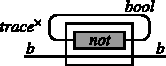
\includegraphics{diagrams/not_trace.pdf}
}
\end{center}
As motivated earlier, it is clearly impossible for the constraint
implied by {{trace*}} to be satisfied as a boolean value {{v}} can
never be the same as its negation. Thus there is no incoming value of
type {{b}} that can ever go through the circuit. Indeed, if we call
the circuit above {{c}}, then we can calculate that 
{{ evalF c v = emptyset}}. We call such a circuit an 
annihilation circuit.
\end{example}

Every relation is clearly reversible by simply swapping the input and
output components of every pair, i.e., if {{r = {[ (a,b), ... ]} }}
then the inverse of {{r}} is simply {{ {[ (b,a), ... ]} }}. 

\begin{proposition}[Logical Reversibility]
\label{prop:logrev-tracet}
For all combinators {{c : b1 <-> b2}} and values {{v1 : b1}} and 
{{v2 : b2}} we have if {{v2 in (evalF c v1)}} then 
{{v1 in (evalB c v2)}}.
\end{proposition}

An interesting point to ponder is what happens to \emph{information}
in circuits like {{annihilate}}? We return to this point later.

%%%%%%%%%%%%%%%%%%%%%%%%%%%%%%%%%%%%%%%%%%%%%%%%%%%%%%%%%%%%%%%%%%%%%%%%%%%%%%%%%
\section{(Finite) Relational Programming}
\label{ch3:sec:lp}

Relational programming leverages set-theoretic relations and their
composition to express computational tasks in a declarative way. For
instance, consider this example:

{{parent = {[ (A,B), (B,C), (A,D) ]} }}

{{grandparent = parent (o) parent}}

\noindent The example defines a relation {{parent}} specified using a
set of tuples and another relation {{grandparent}} specified using the
composition of two parent relations. If we wrote this example in a
relational language (e.g., Prolog) and we executed the query
{{grandparent(A)}}, we would get the answer {{ {[C]} }}.

It turns out that with the addition of the multiplicative trace, and
the move to relations motivated in the previous section, we can
express relational programming. We illustrate the idea using a
complete example. 

Consider the relation {{R}} on booleans given by:

{{ {[(false,false), (false,true), (true,false) ]}. }}

We show how to define a combinator {{c_R}} whose semantics is such that:

%subcode{opsem} include main
%! columnStyle = rcl
% evalF c_R false &=& {[ false, true ]} 
% evalF c_R true &=& {[ false ]} 

The key idea is to find a combinator {{cInner : (a * bool) <-> (a * bool)}}
for some type {{a}} such that {{trace* cInner}} is the desired combinator
{{c_R}}. A little experimentation shows that we get the desired behavior
if {{cInner}} is chosen to behave as follows:

%subcode{opsem} include main
%! columnStyle = rcl
% evalF cInner ((false,false),false) &=& ((false,false),false) 
% evalF cInner ((false,true),false) &=& ((false,true),true) 
% evalF cInner ((false,true),true) &=& ((false,true),false) 
% evalF cInner ((false,false),true) &=& ((true,false),true) 
% evalF cInner ((true,false),false) &=& ((true,true),false) 
% evalF cInner ((true,false),true) &=& ((true,true),true) 
% evalF cInner ((true,true),false) &=& ((true,false),false) 
% evalF cInner ((true,true),true) &=& ((false,false),true) 

In the first three lines, the first argument is a fixed point and hence the
multiplicative trace would map the second input to the second output
producing the desired relation. In the remaining five cases, the first
argument is not a fixed point and hence all these cases would be rejected as
solutions to the constraint imposed by the multiplicative trace. It simply
remains to find the actual realization of {{cInner}} that would produce the
behavior above. One can infer the following implementation:

%subcode{opsem} include main
%! columnStyle = rcl
% cInner &:& (bool * bool) * bool <-> (bool * bool) * bool
% cInner &=& sym (swap* (;) assocl* (;) (cnot (*) id) (;) assoct* (;) swap* (;) 
%        &&  toffoli (;) ((swap* (;) cnot (;) swap*) (*) id) (;)
%        &&  toffoli (;) (assocr* (;) swap* (;) toffoli (;) swap* (;) assocl*) (;)
%        &&  toffoli (;) (cnot (*) id))
%     
% c_R &:& bool <-> bool
% c_R &=& trace* cInner

The above example should convince the reader that the language {{langRev}}
with multiplicative trace is expressive enough to model finite relational
programming. We will not prove this claim. We develop an even more
substantial example: a SAT solver.

%%%%%%%%%%%%%%%%%%%%%%%%%%%%%%%%%%%%%%%%%%%%%%%%%%%%%%%%%%%%%%%%%%%%%%%%%%%%%%%%%
\section{Solving Constraints}
\label{ch3:sec:constraints}

A large class of constraint satisfaction problems can be expressed
using multiplicative traces. We illustrate the main ideas with the
implementation of a SAT solver.

In the usual setting, an instance of SAT is a function~{{f}} which,
when given some boolean inputs, returns {{true}} or {{false}}. The
function returns {{true}} when the inputs satisfy the constraints
imposed by the structure of {{f}} and a solution to the SAT problem is
the set of all inputs on which {{f}} produces {{true}}. The basic idea
of our construction is to generalize the annihilation circuit from
Ex.~\ref{ch3:ex;annihilation} to only annihilate values that fail to
satisfy the constraints represented by the SAT instance {{f}}. To
achieve this goal, we must however deal with several important
details.

First, because we are in a reversible world, our instance of SAT must be
expressed as an isomorphism: this is easily achieved by the construction
which embeds any boolean function {{f}} into a reversible one {{iso_f}} with
a larger domain and range.  Given such a reversible function {{iso_f}} which
represents a SAT instance, we first construct the circuit below:

\begin{center}
\scalebox{1.2}{
  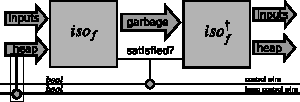
\includegraphics{diagrams/sat2.pdf}
}
\end{center}  

As shown in the circuit, the reversible SAT instance {{iso_f}} takes
two sets of values and produces two outputs. The incoming values
labeled \textsf{inputs} are the inputs we need to test for
satisfiability. The other incoming values labeled \textsf{heap} are
the additional inputs needed to embed the original SAT instance {{f}}
into a reversible function. If these \textsf{heap} values are all
initialized to {{false}}, the output wire \textsf{satisfied?}
corresponds to the output that {{f}} would have produced on
\textsf{inputs}. The other outputs labeled \textsf{garbage} are not
needed for their own sake but they are important because they are used
as inputs to the adjoint of {{iso_f}} to reproduce the inputs exactly,
in anticipation of closing the loop with {{trace*}}.

To summarize, the top half of the circuit is the identity function
except that we have also managed to produce a boolean wire labeled
\textsf{satisfied?} that tells us if the inputs satisfy the desired
constraints. We can take this boolean value and use it to decide
whether to negate the bottom wire (labeled \textsf{control
  wire}). Specifically, if the inputs do \emph{not} satisfy {{f}}, the
control wire is negated. The last wire labeled \textsf{heap control
  wire} is negated if the heap values do not have the right initial
values, i.e., are not all {{false}}.

Let us call the above construction {{sat_f}}. If we now close the loop
using {{trace*}}, two things should happen:
\begin{itemize}
\item configurations in which the \textsf{heap} values are not all
  {{false}} will be annihilated;
\item configurations in which the \textsf{inputs} do not satisfy {{f}}
  will cause the \textsf{satisfied?} wire to be negated and hence will
  also be annihilated.
\end{itemize}
In other words, the only configurations that will survive are the ones in
which the \textsf{inputs} satisfy {{f}}. We simply need to arrange to
\emph{clone} these values and produce them as the output of the whole
circuit. The final construction is therefore:

\begin{center}
\scalebox{1.5}{
  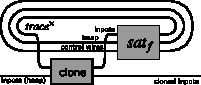
\includegraphics{diagrams/sat3.pdf}
}
\end{center}  

To make the previous discussion concrete, we present a small, but
complete, example. In our example, the SAT instance {{f}} is tiny: it
takes two inputs. This function is embedded into a reversible function
{{iso_f}} of type 
{{((bool * bool) * bool) <-> ((bool * bool) * bool)}} where the last
input represents the heap and the first two outputs represent the garbage. 
The realization of {{sat_f}} given below is parametrized by such 
a function {{iso_f}}. The inputs to {{sat_f}} are 
\textsf{heap control}, \textsf{control}, \textsf{heap}, \textsf{input-1}, and 
\textsf{input-2}. Its operation is simple: if the \textsf{heap} is {{true}}, 
\textsf{heap control} is negated, and if the last output of {{iso_f}} 
is {{false}}, \textsf{control} is negated:

%subcode{opsem} include main
%! columnStyle = rcl
% sat_f &:& ((((bool * bool) * bool) * bool) * bool) <-> ((((bool * bool) * bool) * bool) * bool)
% sat_f &=& ((swap* (*) id) (*) id) (;) 
% && ((assocl* (*) id) (*) id) (;) 
% &&   (((cnot (*) id) (*) id) (*) id) (;) 
% &&   assocr* (;) 
% &&   (assocr* (*) id) (;) 
% &&   (swap* (*) id) (;) 
% &&   assocr* (;) 
% &&   (id (*) assocl*) (;) 
% &&   (id (*) isof) (;) 
% &&   swap* (;) 
% &&   assocr* (;) 
% &&   (id (*) (id (*) swap*)) (;) 
% &&   (id (*) assocl*) (;) 
% &&   (id (*) ((inot (*) id) (*) id)) (;)
% &&   (id (*) (cnot (*) id)) (;) 
% &&   (id (*) ((inot (*) id) (*) id)) (;)
% &&   (id (*) assocr*) (;) 
% &&   (id (*) (id (*) swap*)) (;) 
% &&   assocl* (;)
% &&   swap* (;)
% &&   (id (*) Sym isof) (;) 
% &&   (id (*) assocr*) (;) 
% &&   assocl* (;) 
% &&   assocl* 

Given the construction of {{sat_f}} we can build the full solver as
follows. The overall input is the cloning heap. The combinator given
to {{trace*}} takes the cloning heap and the inputs flowing around the
loop and produces two copies of these inputs. One copy is produced as
the overall output and another is fed back around the loop. 

%subcode{opsem} include main
%! columnStyle = rcl
% solve_f &:& bool * bool <-> bool * Bool
% solve_f &=& trace* (
% && (assocr* (*) id) (;) 
% && assocr* (;)
% && (id (*) swap*) (;)
% && assocl* (;)
% && (assocr* (*) id) (;)
% && (clone2 (*) id) (;)
% && swap* (;)
% && (swap* (*) id) (;)
% && ((swap* (*) id) (*) id) (;)
% && assocl* (;)
% && assocl* (;)
% && (sat_f (*) id) (;)
% && (assocr* (*) id) (;)
% && (swap* (*) id) (;) 
% && ((id (*) swap*) (*) id) (;)
% && (assocl* (*) id) (;)
% && ((id (*) swap*) (*) id))

We can test our {{solve_f}} combinator using several SAT
instances. Here are two possible instances. The first instance is
satisfied by {{(false,false)}} and the
second is satisfied by {{(false,true)}} and {{(true,true)}}.

%subcode{opsem} include main
%! columnStyle = rcl
% iso_{f_1} &:& ((bool * bool) * bool) <-> ((bool * bool) * bool)
% iso_{f_1} &=& (assocr* (;) swap* (;) toffoli (;) swap* (;) assocl*) (;)
% && (((swap+ (*) id) (*) id) (;) toffoli (;) ((swap+ (*) id) (*) id)) (;) 
% && (id (*) swap+)
% 
% iso_{f_2} &:& ((bool * bool) * bool) <-> ((bool * bool) * bool)
% iso_{f_2} &=& toffoli

It can indeed be verified using the semantics that the {{solve_f}}
combinators instantiated with the SAT instances produce the expected
results. 

%%%%%%%%%%%%%%%%%%%%%%%%%%%%%%%%%%%%%%%%%%%%%%%%%%%%%%%%%%%%%%%%%%%%%%%%%%%%
\section{The Idea}

Our development so far has been fairly traditional in the sense that
we have applied well-known type constructions and semantic techniques
to a language of isomorphisms. In this chapter, we begin to explore
more novel ideas. 

One of the benefits of having a reversible language in which
information is preserved is that essentially every construction can be
considered in reverse. We begin in this chapter by considering the
idea of \emph{fractional types} which are dual to product types. We
call the resulting language {{langRevTF}}.

We have already seen in Sec.~\ref{sec:trace} that the multiplicative
trace can be viewed as performing some kind of ``division'' on
types. Recall that given a combinator {{c : b * b1 <-> b * b2}}, we
have {{trace* c : b1 <-> b2}} which \emph{cancels} the type {{b}}.
Our plan is to make this ``division operation'' a first-class one. In
other words, we introduce a new type construction --- a fractional
type {{1/b}} --- that allows us to cancel any type {{b}} in a
multiplicative context, i.e., that satisfies the isomorphism:

%subcode{bnf} include main
%  eps*_b :& 1/b * b ~~<->~~ 1 &: eta*_b

Given this fractional type and its associated isomorphism, we can
perform the cancellation implicit in {{trace*}} as follows. 
Let {{ c :  b * b1 <-> b * b2 }} be given and consider the 
following sequence of type isomorphisms:

%subcode{bnf} include main
%  b1 &<->& 1 * b1 & (uniti)
%     &<->& (1/b * b) * b1 & (eta*_b)
%     &<->& 1/b * (b * b1) & (assocr*)
%     &<->& 1/b * (b * b2) & (c)
%     &<->& ((1/b * b) * b2) & (assocl*)
%     &<->& (1 * b2) & (eps*_b)
%     &<->& b2 & (unite*)

\noindent This sequence of isomorphisms, at least at the type level,
seems to produce the desired {{trace*}}. We will confirm this in the
next section after we introduce the formal syntax and semantics. For
now, we provide an intuitive understanding of the type {{1/b}}.

If {{v : b}}, we define the value {{1/v : 1/b}} and these are the only
values of type~{{1/b}}. Since there are no values of type {{0}}, this
means that {{1/0}} is also an empty type. Generally, we think of a
value like {{1/false}} as a \emph{first-class constraint} that can
only be satisfied if it is matched with an actual value {{false}}. So
intuitively, {{trace*}} allowed us to implicitly introduce constraints
in our model which we now make explicit and first-class entities. This
makes the language much more expressive: as we show in this chapter,
it essentially gains the expressive power to model higher-order
relations.

%%%%%%%%%%%%%%%%%%%%%%%%%%%%%%%%%%%%%%%%%%%%%%%%%%%%%%%%%%%%%%%%%%%%%%%%%%%%
\section{The Language: {{langRevTF}} }

We extend {{langRevT}} with fractional types, fractional values, and
two combinators {{eta*_b}} and {{eps*_b}} motivated above.  We provide the
full syntactic and semantic definitions for the language below.

\begin{definition}[Syntax of {{langRevT}}]
\label{def:langRevT}
The syntax of types, values, and combinators, is:
%subcode{bnf} include main
% natural numbers, n 
% value types, b ::= 0 | 1 | b+b | b*b | 1/b | bool | nat 
% values, v ::= () | left v | right v | (v,v) | 1/v | true | false | n
%
% combinator types, t ::= b <-> b
% isomorphisms, iso ::= zeroe | zeroi | swap+ | assocl+ | assocr+ 
%                   &|& unite | uniti | swap* | assocl* | assocr* 
%                   &|& dist0 | factor0 | dist | factor 
%                   &|& foldB | unfoldB | foldN | unfoldN
%                   &|& eta*_b | eps*_b
% combinators, c ::= iso | id | sym c | c (;) c | c (+) c | c (*) c 
%                   &|& trace+ c | trace* c
\end{definition}

The denotation of types is extended with a clause for fractional types.

\begin{definition}[Denotation of Types {{ [[b]] }}]
\label{chx:def:denot}
Each type denotes a set of values as follows:
\[\begin{array}{rcl}
\llbracket 0 \rrbracket &=& \emptyset \\
\llbracket 1 \rrbracket &=& \{ () \} \\
\llbracket b_1 + b_2 \rrbracket &=& \{ \mathit{left}~v ~|~ v \leftarrow \llbracket b_1 \rrbracket \}
           \cup \{ \mathit{right}~v ~|~ v \leftarrow \llbracket b_2 \rrbracket \} \\
\llbracket b_1 \times b_2 \rrbracket &=& \{ (v_1,v_2) ~|~ v_1 \leftarrow \llbracket b_1 \rrbracket, 
           v_2 \leftarrow \llbracket b_2 \rrbracket \} \\
\llbracket 1/v \rrbracket &=& \{ 1/v ~|~ v \leftarrow \llbracket b \rrbracket \} \\
\llbracket \mathit{bool} \rrbracket &=& \{ \mathit{true}, \mathit{false} \} \\
\llbracket \mathit{nat} \rrbracket &=& \{ 0, 1, 2, \ldots \} 
\end{array}\]
\end{definition}

As usual, the semantics of {{langRevTF}} is given using two mutually
recursive interpreters: one going forward and one going backwards. As
motivated and explained in Sec.~\ref{sec:trace}, each combinator denotes
a \emph{relation} and hence the result of applying a combinator to a
value generally returns a \emph{set} of values. We only show the new
cases for {{eta*_b}} and {{eps*_b}}.

\begin{definition}[Operational semantics for {{langRevTF}}]
\label{def:operational-langRevTF}
Given a program {{c : b1 <-> b2}} in {{langRev}}, we can run it in the
forward direction by supplying it with a value {{ v1 : b1 }} and in
the backwards direction by supplying it with a value {{v2 : b2}}. 

\paragraph*{Forward Evaluator (clauses for {{eta*_b}} and {{eps*_b}}): }

%subcode{opsem} include main
%! columnStyle = rcl
% evalF ~eta*_b () &=& Union_{v in [[b]]} ~{[ (1/v,v) ]}
% evalF ~eps*_b (1/v,v) &=& {[ () ]} 
% evalF ~eps*_b (1/v1,v2) &=& emptyset, where v1 /= v2

\paragraph*{Backwards Evaluator (clauses for {{eta*_b}} and {{eps*_b}}): }

%subcode{opsem} include main
%! columnStyle = rcl
% evalB ~eta*_b (1/v,v) &=& {[ () ]} 
% evalB ~eta*_b (1/v1,v2) &=& emptyset, where v1 /= v2
% evalB ~eps*_b () &=& Union_{v in [[b]]} ~{[ (1/v,v) ]}
\end{definition}

The language {{langRevT}} is still logically reversible. 

\begin{proposition}[Logical Reversibility]
\label{chx:prop:logrev-tracep}
For all combinators {{c : b1 <-> b2}} and values {{v1 : b1}} and 
{{v2 : b2}} we have {{v2 in (evalF c v1)}} iff
{{v1 in (evalB c v2)}}.
\end{proposition}

%%%%%%%%%%%%%%%%%%%%%%%%%%%%%%%%%%%%%%%%%%%%%%%%%%%%%%%%%%%%%%%%%%%%%%%%%%%%
\section{Expressiveness}

Fractional types and values add considerable expressiveness to our
language.

%%%%%%%%%%%%
\subsection{Trace}

With fractionals, the trace operator becomes expressible:

%subcode{opsem} include main
%! columnStyle = rcl
% trace*_b &:& ((b * b1) <-> (b * b2)) -> (b1 <-> b2)
% trace*_b c &=& uniti (;) (eta*_b (*) id) (;) assocr* (;) 
%            && (id (*) c) (;) assocl* (;) (eps*_b (*) id) (;) unite

Let's use the semantics to calculate the result of applying
{{trace*_{bool} (not (*) id)}} to {{false}}. We start
with the set {{ {[ false ]} }} which gets transformed as follows:
%subcode{opsem} include main
%! columnStyle = ll
% {[ ((),false) ]}  & (uniti)
% {[ ((1/false,false),false), ((1/true,true),false) ]} & (eta*_{bool})
% {[ (1/false, (false,false)), (1/true,(true,false)) ]} & (assocr*)
% {[ (1/false, (true,false)), (1/true,(false,false)) ]} & (not (*) id)
% {[ ((1/false,true),false), ((1/true,false),false) ]} & (assocl*)
% emptyset & eps*_{bool}

And indeed this is the annhiliation circuit from
Ex.~\ref{ch3:ex;annihilation}.

%%%%%%%%%%%%
\subsection{First-Class Relations}

With fractional types, we can turn define a value that denotes a
first-class function or relation. Indeed a value of type {{1/b1 * b2}}
is a pair of a \emph{constraint} that can only be satisfied by some
{{v1 : b1}} and a value {{v2 : b2}}. In other words, it corresponds to
a function or relation which when given matched with a value {{v1 : b1}} 
``releases'' the value {{v2 : b2}}. In the remainder of the book, we 
introduce this abbreviation:

%subcode{bnf} include main
%  b1 :-* b2 ::= 1/b1 * b2

What is remarkable is that we can systematically turn any combinator
{{c : b1 <-> b2}} into a (constant) value of type {{b1 :-* b2}} as
shown below:

%subcode{opsem} include main
%! columnStyle = rcl
% name &:& (b1 <-> b2) -> (1 <-> (b1 :-* b2))
% name c &=& eta*_{b1} (;) (id (*) c)

As a simple example, consider the combinator 
{{name not : 1 <-> (bool :-* bool)}}. Applying this 
combinator to {{ () }} evaluates as follows:

%subcode{opsem} include main
%! columnStyle = ll
% {[ () ]}  & 
% {[ (1/false,false), (1/true,true) ]} & eta*_{bool}
% {[ (1/false,true), (1/true,false) ]} & id (*) not

\noindent In other words, the result of applying the combinator to {{ () }}
is a value that represents the boolean negation function. 

%%%%%%%%%%%%
\subsection{Higher-Order Relations}

We are now a small step to implementing various higher-order
combinators that manipulate functions or relations. In particular, we
can \emph{apply} and \emph{compose} values representing relations as
shown below:

%subcode{opsem} include main
%! columnStyle = rcl
% apply &:& (b1 :-* b2) * b1 <-> b2
% apply &=& swap* (;) assocl* (;) (swap* (*) id) (;) (eps*_{b1} (*) id) (;) unite

\noindent At the type level, the computation proceeds as follows:
%subcode{bnf} include main
%  (b1 :-* b2) * b1 &=& (1/b1 * b2) * b1 & 
%     &<->& b1 * (1/b1 * b2) & (swap*)
%     &<->& (b1 * 1/b1) * b2) & (assocl*)
%     &<->& (1/b1 * b1) * b2) & (swap* (*) id)
%     &<->& 1 * b2 & (eps*{b1} (*) id)
%     &<->& b2 & (unite)

\noindent Intuitively, we simply match the incoming argument of type {{b1}} with
the constraint encoded by the function. If they match, they cancel
each other and the value of type {{b2}} is exposed with no
constraints. Otherwise, the mismatched values are \emph{annihilated}.

Function or relation composition is only slightly more involved:

%subcode{opsem} include main
%! columnStyle = rcl
% compose &:& (b1 :-* b2) * (b2 :-* b3) -> (b1 :-* b3)
% compose &=& assocr* (;) (id (*) (assocl* (;) (swap* (*) id) (;) (eps*_{b2} (*) id) (;) unite))

\noindent Again, at the type level, the computation proceeds as follows:

%subcode{bnf} include main
%  (b1 :-* b2) * (b2 :-* b3) &=& (1/b1 * b2) * (1/b2 * b3) & 
%     &<->& (1/b1 * (b2 * (1/b2 * b3)) & (assocr*)
%     &<->& (1/b1 * ((b2 * 1/b2) * b3) & (assocl*)
%     &<->& (1/b1 * ((1/b2 * b2) * b3) & (assocl*)
%     &<->& (1/b1 * (1 * b3) & (eps*_{b2})
%     &<->& (1/b1 * b3) & (unite)
%     &=& b1 :-* b3

%%%%%%%%%%%%
\subsection{Duality}

The final remarkable property of fractional types is that they
constitute, a form of self-inverse negation. In particular, we have:

%subcode{opsem} include main
%! columnStyle = rcl
% doubleNeg &:& b <-> 1/(1/b)
% doubleNeg &=& uniti (;) (eta*_{1/b} (*) id) (;) assocr* (;) (id (*) eps*_b) (;) swap* (;) unite

\noindent At the type level, this computation proceeds as follows:

%subcode{bnf} include main
%  b &<->& (1 * b) & (uniti)
%    &<->& (1/(1/b) * 1/b) * b & (eta*_{1/b} (*) id)
%    &<->& 1/(1/b) * (1/b * b) & (assocr*)
%    &<->& 1/(1/b) * 1 & (id (*) eps*_b)
%    &<->& 1 * 1/(1/b) & (swap*)
%    &<->& 1/(1/b) & (unite)

What is interesting about this isomorphism is that it holds for all
types {{b}}, and in particular we have {{0 <-> 1/(1/0)}}.




\bibliographystyle{splncs03} 
\bibliography{cites}
\end{document}

